\section{Hadoop Cluster}
\subsection{Requirements}
Hadoop itself does not have any explicit hardware requirements, and is able to run on mainst

Hadoop also very few software requirements and is able to run on both Microsoft Windows and varieties of GNU/Linux. Use of Hadoop on a Windows environment is recommended only as a development platform, as Hadoop has not been well tested as a production platform for Windows. Both development and production have been tested using GNU/Linux environments, and is the recommended for use of Hadoop.

Hadoop only has two explicit software requirements: Java\footnote{\url{http://www.java.com/}} and ssh\footnote{\url{http://www.openssh.com/}}. Hadoop launches each of the services required to manage a cluster as Java processes, and as such requires the Java Runtime Environment 1.6.x to be present. As programs developed using Giraph are written in Java, the Java Development Kit is also required, and includes the Java Runtime Environment. Ssh is required, with sshd running on all nodes, to allow the NameNode to manage all nodes within the cluster. 

Giraph has a few extra requirements of its own. It requires specific versions of Hadoop, Hadoop 0.20.203 or higher, which have security changes applied to them. At the time of the project commencement, Hadoop 0.20.205 had been released\footnote{\date{17th October 2011} - \url{http://hadoop.apache.org/common/releases.html}} as the latest version with the required security changes, and as such has been the version with which development of the project has been made with. During the development of the project, Hadoop reached version 1.0.0\footnote{\date{27th December 2011} - \url{http://hadoop.apache.org/common/releases.html}} but we chose to remain with the existing version of Hadoop so as not to introduce any conflicts with any possible deprecations or changes brought about by the newer version.

Giraph also requires Maven 3\footnote{\url{http://maven.apache.org/}} to be installed to compile the Giraph source code into a usable JAR for submitting jobs with to Hadoop.

\subsection{Single-Node Cluster}
For development purposes single-node cluster \cite{nollsingle}

\begin{figure}[htbp]
  \centering
    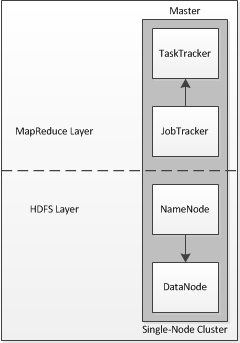
\includegraphics{./img/singlenode}
  \caption{Single-node Hadoop cluster \cite{nollsingle}.}
  \label{fig:singlenode}
\end{figure}

\subsection{Two-Node Cluster}
\cite{nollmulti}

\begin{figure}[htbp]
  \centering
    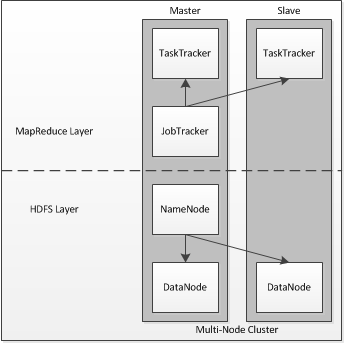
\includegraphics{./img/twonode}
  \caption{Two-nodes Hadoop cluster \cite{nollmulti}.}
  \label{fig:twonode}
\end{figure}

\subsection{Multi-Node Cluster}
At request, a nine machine Hadoop cluster was set up for use during this project in the department of computer science. This cluster composed a master head-node, {\tt hadoopmaster}, and eight slave-nodes, {\tt hadoop\{0-7\}}. 

Being the master, {\tt hadoopmaster} runs the NameNode, JobTracker and SecondaryNameNode processes. Each of the slave-nodes run the DataNode and TaskTracker processes.

HERE WILL BE SOME TECHNICAL SPECS ABOUT THE HADOOP CLUSTER IN THE DEPARTMENT

We did not have direct access to the Hadoop cluster, and were required to {\tt ssh} to a machine located within the department, before {\tt ssh}ing from this machine into the Hadoop cluster. This added an extra level of complexity to access the Hadoop cluster , yet was resolved though use of ssh-keys to allow this \emph{machine-in-the-middle} to send and receive files from hadoopmaster with requiring a password.

\subsubsection{Issues}
One major issue which surfaced when we gained access to the Hadoop cluster in the department of computer science, relating to using Giraph with more than one worker. When a Giraph job is submitted to the cluster using more than one worker, each node which gets used by the job starts a listener which receives messages sent. However, whilst Hadoop jobs submitted to the cluster were able to make use of all nodes within the cluster, Giraph jobs were only able to use one worker, and therefore one node, otherwise an error similar to Listing \ref{lst:girapherror}.

\lstset{language=Java,caption={Giraph error message},label=lst:girapherror,tabsize=2,breaklines=true,breakatwhitespace=true,frame=single}
\begin{lstlisting}[float]
java.net.ConnectException: Call to hadoop6.deepthought.hpsg.dcs.warwick.ac.uk/10.131.56.209:30002 failed on connection exception: java.net.ConnectException: Connection refused
\end{lstlisting}

This error was indicating that there was something wrong with the network configuration, with the most likely problem being that the ports listed in the errors were closed due to a firewall, or similar. However, after some investigation, it turned out that the ports were not blocked and that there was some other issue occuring. Browsing through the user mailing list for Giraph, it became apparent that another user of Giraph was producing the same errors as our cluster\footnote{\url{http://mail-archives.apache.org/mod_mbox/incubator-giraph-user/201112.mbox/\%3C4ED9DDAC.4070208@apache.org\%3E}}. The issue with the use of Giraph on the cluster is how the workers work out which IP address they should listen on, which happens in a different manner to how Hadoop operates, hence why Hadoop jobs would successfully execute whilst Giraph jobs would not. The fix was to remove the mapping from {\tt 127.0.0.1} to {\tt localhost} from the {\tt /etc/hosts} file. With this change made, we were able to successfully able to execute Giraph jobs, making full use of the cluster available.

Another issue which occurred with the cluster is that node {\tt hadoop3} began to produce error messages as show in Listing \ref{lst:hadoop3error}. What was confusing about this error was that all slave nodes, {\tt hadoop\{0-7\}}, are identical in setup and configuration, so for only {\tt hadoop3} to produce serious errors such as this was strange.

\lstset{language=Java,caption={hadoop3 error message},label=lst:hadoop3error,tabsize=2,breaklines=true,breakatwhitespace=true,frame=single}
\begin{lstlisting}[float]
java.lang.Throwable: Child Error
        at org.apache.hadoop.mapred.TaskRunner.run
        (TaskRunner.java:271)
Caused by: java.io.IOException: Task process exit with nonzero status of 134.
        at org.apache.hadoop.mapred.TaskRunner.run
        (TaskRunner.java:258)

attempt_201204171536_0005_m_000005_0: #
attempt_201204171536_0005_m_000005_0: # A fatal error has been detected by the Java Runtime Environment:
attempt_201204171536_0005_m_000005_0: #
attempt_201204171536_0005_m_000005_0: #  SIGSEGV (0xb) at pc=0x00007f4035255dbc, pid=25782, tid=139913655404288
attempt_201204171536_0005_m_000005_0: #
attempt_201204171536_0005_m_000005_0: # JRE version: 7.0_02-b13
attempt_201204171536_0005_m_000005_0: # Java VM: Java HotSpot(TM) 64-Bit Server VM (22.0-b10 mixed mode linux-amd64 compressed oops)
attempt_201204171536_0005_m_000005_0: # Problematic frame:
attempt_201204171536_0005_m_000005_0: # C  [libc.so.6+0x7fdbc]  memcpy+0x4cc
attempt_201204171536_0005_m_000005_0: #
attempt_201204171536_0005_m_000005_0: # Failed to write core dump. Core dumps have been disabled. To enable core dumping, try "ulimit -c unlimited" before starting Java again
attempt_201204171536_0005_m_000005_0: #
attempt_201204171536_0005_m_000005_0: # An error report file with more information is saved as:
attempt_201204171536_0005_m_000005_0: # /home/hduser/hadoop/tmp/mapred/local/taskTracker/hduser/
jobcache/job_201204171536_0005/
attempt_201204171536_0005_m_000005_0/work/
hs_err_pid25782.log
attempt_201204171536_0005_m_000005_0: # [ timer expired, abort... ]
\end{lstlisting}

The approach we took to remedy this was to remove {\tt hadoop3} from operating within the cluster. As {\tt hadoop3} was also a DataNode, the HDFS needed to re-replicate the data held on {\tt hadoop3} across the other seven nodes before they could continue operating as the cluster.